\documentclass{beamer}
\mode<presentation>
\usepackage{amsmath}
\usepackage{amssymb}
%\usepackage{advdate}
\usepackage{adjustbox}
\usepackage{subcaption}
\usepackage{enumitem}
\usepackage{multicol}
\usepackage{listings}
\usepackage{url}
\usepackage{tikz}
\usepackage{tzplot}
\def\UrlBreaks{\do\/\do-}
\usetheme{Boadilla}
\usecolortheme{lily}
\setbeamertemplate{footline}
{
  \leavevmode%
  \hbox{%
  \begin{beamercolorbox}[wd=\paperwidth,ht=2.25ex,dp=1ex,right]{author in head/foot}%
    \insertframenumber{} / \inserttotalframenumber\hspace*{2ex} 
  \end{beamercolorbox}}%
  \vskip0pt%
}
\setbeamertemplate{navigation symbols}{}

\providecommand{\nCr}[2]{\,^{#1}C_{#2}} % nCr
\providecommand{\nPr}[2]{\,^{#1}P_{#2}} % nPr
\providecommand{\mbf}{\mathbf}
\providecommand{\pr}[1]{\ensuremath{\Pr\left(#1\right)}}
\providecommand{\qfunc}[1]{\ensuremath{Q\left(#1\right)}}
\providecommand{\sbrak}[1]{\ensuremath{{}\left[#1\right]}}
\providecommand{\lsbrak}[1]{\ensuremath{{}\left[#1\right.}}
\providecommand{\rsbrak}[1]{\ensuremath{{}\left.#1\right]}}
\providecommand{\brak}[1]{\ensuremath{\left(#1\right)}}
\providecommand{\lbrak}[1]{\ensuremath{\left(#1\right.}}
\providecommand{\rbrak}[1]{\ensuremath{\left.#1\right)}}
\providecommand{\cbrak}[1]{\ensuremath{\left\{#1\right\}}}
\providecommand{\lcbrak}[1]{\ensuremath{\left\{#1\right.}}
\providecommand{\rcbrak}[1]{\ensuremath{\left.#1\right\}}}
\theoremstyle{remark}
\newtheorem{rem}{Remark}
\newcommand{\sgn}{\mathop{\mathrm{sgn}}}
\providecommand{\res}[1]{\Res\displaylimits_{#1}} 
\providecommand{\norm}[1]{\lVert#1\rVert}
\providecommand{\mtx}[1]{\mathbf{#1}}
\providecommand{\fourier}{\overset{\mathcal{F}}{ \rightleftharpoons}}
%\providecommand{\hilbert}{\overset{\mathcal{H}}{ \rightleftharpoons}}
\providecommand{\system}{\overset{\mathcal{H}}{ \longleftrightarrow}}
	%\newcommand{\solution}[2]{\textbf{Solution:}{#1}}
%\newcommand{\solution}{\noindent \textbf{Solution: }}
\providecommand{\dec}[2]{\ensuremath{\overset{#1}{\underset{#2}{\gtrless}}}}
\newcommand{\myvec}[1]{\ensuremath{\begin{pmatrix}#1\end{pmatrix}}}
\let\vec\mathbf

\lstset{
%language=C,
frame=single, 
breaklines=true,
columns=fullflexible
}

\numberwithin{equation}{section}

\title{Assignment 1}
\author{Ingilela Rohith \\ EE19BTECH11005}

\date{\today} 
\begin{document}

\begin{frame}
\titlepage
\end{frame}

\section*{Outline}
\begin{frame}
\tableofcontents
\end{frame}
\section{Problem}
\begin{frame}
\frametitle{Problem Statement}
Construct a triangle, given its base, a base angle and sum
of other two sides. \\
\vspace{10pt}

Given the base BC, a base angle, say ∠B and the sum AB + AC of the other two sides of a triangle ABC, you are required to construct it.
\begin{center}
\begin{tikzpicture}
% triangle
\tzcoors(0,0)(B){$B$}[180](4,0)(C){$C$}[-45](3.5,3)(A){$A$}[45];
\tzpolygon(A){}[b](B){}[r](C){}[sloped,a](A);
% angle marks
\tzanglemark(A)(B)(C){}
\end{tikzpicture}
\end{center}

\end{frame}

\section{Solution}
\begin{frame}
\frametitle{Solution}

Using the cosine formula in $\triangle ABC$,
\begin{equation}
    b^2 = a^2 + c^2 - 2ac Cos B    
\end{equation}
\begin{equation}
    (b + c)(b - c) = a^2 - 2ac Cos B
\end{equation}
\begin{equation}
    or, K(b - c) = a^2 - 2ac Cos B
\end{equation}
\begin{equation}
    \text{where }  K = b + c
\end{equation}
\begin{equation}
    Kb + c (2aCosB - K) = a^2
\end{equation}
\end{frame}

\begin{frame}{}
    Writing (3.4) and (3.5) into matrix form

\begin{equation}
    \begin{pmatrix}
     1 &  1 \\
     K & 2aCosB - K
    \end{pmatrix}
    \begin{pmatrix}
     b \\
     c
    \end{pmatrix}
    =
    \begin{pmatrix}
     K \\
     a^2
    \end{pmatrix}
\end{equation} \\
\vspace{10pt}
Solve matrix (3.6) for 'c' \\
\vspace{10pt}
The coordinates of $\triangle ABC$ can then be expressed as
    \begin{equation}
        \Vec{A} = c
        \begin{pmatrix}
            cos B \\
            sin B
        \end{pmatrix},
        \Vec{B} =
        \begin{pmatrix}
            0 \\
            0
        \end{pmatrix},
        \Vec{C} = 
        \begin{pmatrix}
            a \\
            0
        \end{pmatrix}
    \end{equation}
    
\end{frame}

\section{Code}
\begin{frame}[fragile]
\frametitle{Code}
{\footnotesize
\begin{lstlisting}[language=Python]
import numpy as np
import matplotlib.pyplot as plt
		
def construct_triangle(BC, angle_B, AB_plus_AC):
    a = BC
    K = AB_plus_AC
    B = np.deg2rad(angle_B)

    X = np.array([ [1,  1], [K, 2*a*np.cos(B) - K] ])
    D = np.array([ K, a*a ])
    c = np.linalg.solve(X, D)[1]

    A = (c * np.cos(B), c * np.sin(B))
    B = (0, 0)
    C = (a, 0)

    plt_line(A, B, 'A', 'B')
    plt_line(B, C, 'B', 'C')
    plt_line(C, A, 'C', 'A')
    
\end{lstlisting}
}
\end{frame}
\begin{frame}[fragile]
\frametitle{}
{\footnotesize
\begin{lstlisting}[language=Python]
def plt_pnt(A, label=''):
	plt.plot(A[0], A[1], 'o')
	if label != '':
		plt.text(A[0], A[1], label)
		
def plt_line(A, B, labelA='', labelB='', plt_plts = True):
	plt.plot([A[0],B[0]], [A[1],B[1]], label=labelA+labelB)
	if plt_plts:
		plt_pnt(A, labelA)
		plt_pnt(B, labelB)
		
construct_triangle(7, 75, 13)

plt.grid(), plt.axis('equal')
plt.show()
\end{lstlisting}
}
\end{frame}

\section{Plot}
\begin{frame}
\frametitle{Plot}
The above code plots Fig.\ref{fig:direction_vectors}.
\begin{figure}
\centering
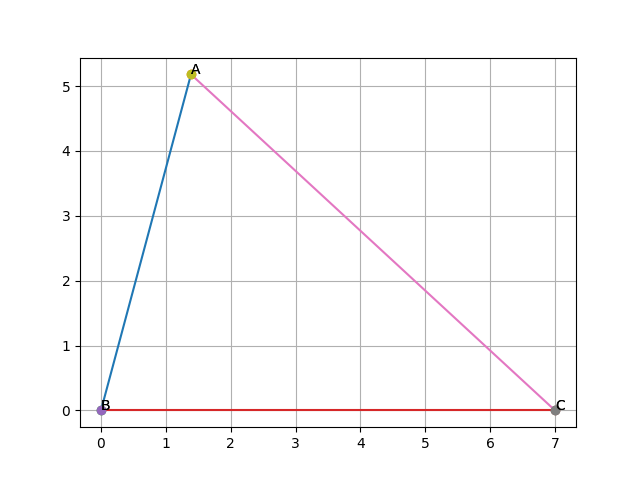
\includegraphics[width=0.75\columnwidth]{Figure_1.png}
\caption{Triangle with BC=7; $\angle$B = 75$^{\circ}$; AB + BC = 13}
\label{fig:direction_vectors}
\end{figure}
\end{frame}

\end{document}